% !TEX root = ../main.tex
\subsubsection{Residuals Improvements}
\label{sssec::residuals_improvements}
    To validate the proposed alignment algorithm, it was applied to the data from Run Group F (RG-F), specifically Run 11983.
    The improvement in residuals is readily apparent when comparing the before and after alignment results, as depicted in figure \ref{fig::res_comparison}.
    It is important to note the difference in scale between the top and bottom plots, which further highlights the significant improvement achieved through the alignment process.

    \begin{figure}[t!]
        \centering\frame{
        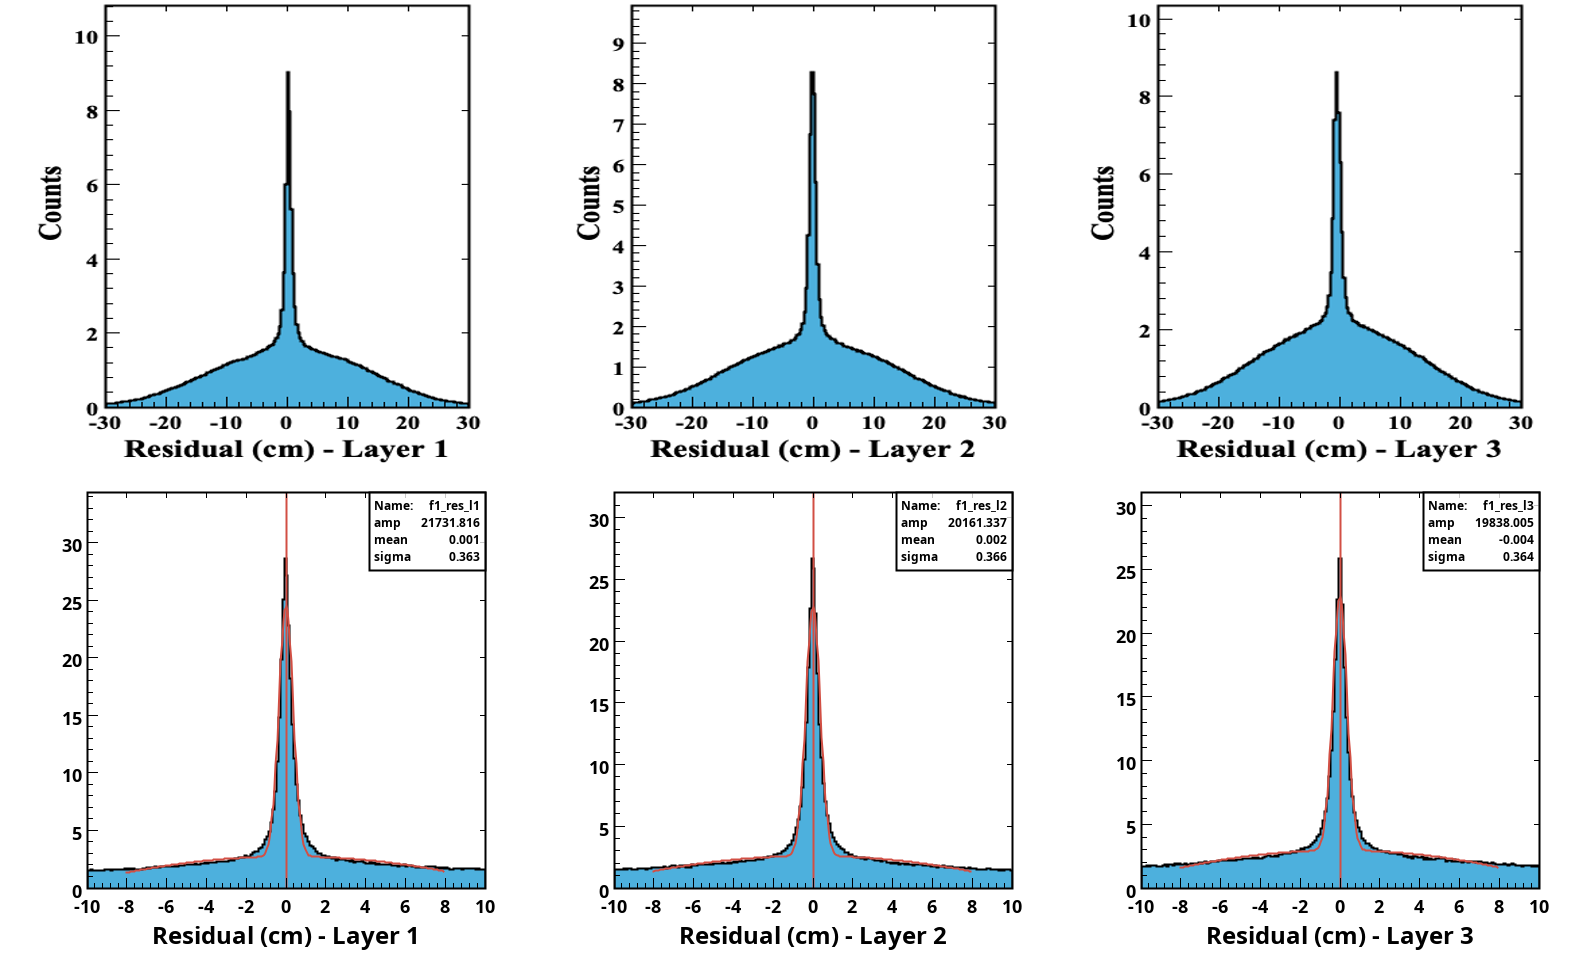
\includegraphics[width=\textwidth]{22res_comparison.png}}
        \caption[Residuals distribution improvement.]{Residuals distribution before (upper image) and after (lower image) alignment.
        Source: \hyperlink{github.com/JeffersonLab/clas12alignment}{CLAS12 alignment software}.}
        \label{fig::res_comparison}
    \end{figure}

    As depicted in the figure, the $z$ and $\phi$ alignment significantly reduces the background, resulting in a higher concentration of residuals around the mean of the distribution.
    Moreover, the $x$ and $y$ alignment effectively aligns the mean of the distribution closer to zero, improving the overall alignment.
    However, for the pitch and yaw alignment, meaningful results could not be obtained.
    This can be attributed to the limited data available from the three layers, combined with the small rotations around the $x$ and $y$ axes, making it challenging to achieve precise alignment.

    To determine the mean and standard deviation ($\sigma$) of the distribution, a Gaussian fit was applied. The parameters of the Gaussian fit are
     \begin{align*}
        \Big( \text{amp} \cdot \text{gaus}(\mu, \sigma) \Big) &+ \Big( p_0 + p_1\cdot x + p_2\cdot x^2 \Big) \\
        \text{gaussian} \hspace{0.8cm} &+ \hspace{1cm} \text{background}
    \end{align*}

    The results obtained are included in the CCDB at:

    \small\href{clasweb.jlab.org/cgi-bin/ccdb/versions?table=/geometry/fmt/alignment}{\texttt{clasweb.jlab.org/cgi-bin/ccdb/versions?table=/geometry/fmt/alignment}}

    Alignment was successfully performed for the data from Run Group M (RG-M), demonstrating that the alignment procedure is not specific to a particular run.
    This indicates the general applicability and effectiveness of the alignment procedure across different runs in the CLAS12 detector.

    The impact of this alignment procedure on the resolution of the entire CLAS12 detector will be further investigated and discussed in the concluding subsection of the section.
